
\section{Word Embedding Experiments}
\label{sec:experiments}

In order to better understand the effects of different parameters on the quality of the final embeddings, we evaluate the multiple parameter combinations of each of the parameter selections outlined in Section \ref{sec:training}. The text corpus for training the embeddings is an Arabic Wikipedia dump from \url{https://dumps.wikimedia.org/arwiki/20150901/} \cite{wiki:xxx}, cleaned by dropping Wikipedia markup, punctuation, and non-Arabic characters. All preprocessing options are precomputed first, generating multiple versions of the Arabic Wikipedia corpus. Then word vectors are trained for each parameterization. The vectors are then run through the evaluation tasks, recording performance statistics.

\subsection{Word Similarity 353}

There are two baseline English models that we use for comparison on the evaluation tasks. The first is an English model trained under the default Word2vec parameterization (skipgram, window of 7, 100 dimensions) on the same number of words as our Arabic models (5 million). The second is the publicly available pre-trained model trained on a 100 billion word Google News Corpus \cite{mikolovdist:2013}. The metric that we choose to base our evaluations on is the Spearman correlation between the model similarity estimates and the evaluation task similarity values. Both models have a high correlation with the evaluation task scores. The Google News vectors has a $0.6979$ Spearman correlation score to the task, providing a high score to aim for. We consider the model trained on 5 million words to be our target baseline for our Arabic word embeddings, with a correlation score of $0.5458$.

Figure \ref{fig:spearplotws353} shows the results of the models on the Word Similarity 353 task \cite{finkelstein:2001,hassan:2009}. In this style of plot, we group the models by the training parameter that most significantly affect scores on the task and provide boxplots for the group's distribution of scores. Here we can see the best performing models were primarily trained using a window of 4 words and preprocessed to tokens. These results show that tokenization is the only method that performs as well as the English baseline, outperforming it \textbf{ADD EXACT CORRELATION HERE}. This improvement can be considered even more significant due to the translation of the task, but it is difficult to quantify how much loss occurred from translation. Interestingly, the unprocessed base text scores higher than lemmatization on this task, possibly due to the comparatively simpler, noun dominated terms in the task. Lemmatization likely over-simplifies the words, while in our similarity task the higher complexity of the terms benefits more from lemmatization. The window size is very interesting, as this parameter is highly dependent on the grammar of the training language. A sentence structure that uses complex words more often has related words nearer to each other than English does, so Arabic word embeddings may benefit from having a smaller window size of 4 to not look beyond the relevant information.

% \begin{wraptable}{l}{0.4\linewidth}
% \begin{center}
% \begin{tabular}{l|l|l|l|l}
% \bfseries Rank & \bfseries Preprocessing & \bfseries Window & \bfseries Size & \bfseries Correlation
% \csvreader[column count=15,head to column names]{results_spearman/ar_similiarity_task_results_ws353_prepared.csv}{}
% {\\\hline\rank&\preprocessing&\wind&\size&\Spearman}
% \end{tabular}
% \caption{Top Results on Arabic Word Similarity 353}
% \label{table:ws353task}
% \end{center}
% \end{wraptable}

% \begin{table}
% \begin{center}
% \begin{tabular}{l|l|l}
% \bfseries Data Set &\bfseries Similarity Correlation & \bfseries Analogy Accuracy
% \csvreader[head to column names]{results_spearman/en_prepared_hybrid.csv}{}
% {\\\hline\csvcoli&\Spearman&\Scores}
% \end{tabular}
% \caption{English Baseline Results}
% \label{table:englishtask}
% \end{center}
% \end{table}

\begin{wrapfigure}{l}{0.5\linewidth}
  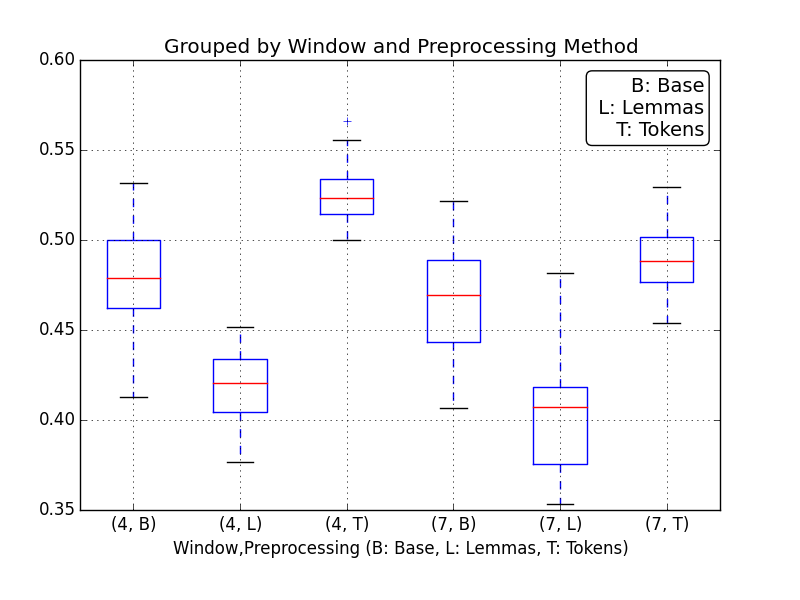
\includegraphics[width=\linewidth]{results_spearman/ar_similiarity_task_results_ws353_spearplot.png}
  \caption{Results on Arabic Word Similarity 353}
  \label{fig:spearplotws353}
\end{wrapfigure}

\subsection{Our Similarity Task}

Figure \ref{fig:spearplot4} show the results of the models on the task we developed. We also computed results for our task using only 1 and 2 fluent Arabic evaluators to obtain similarity scores, which are not shown here but demonstrate identical trends. The Kendall Tau scores between these three rankings are 0.335 between the full set of word pairs and the set with four votes, 0.482 between the full set and the set with two or more votes, and 0.572 between the task with two votes and the task with four votes (all highly significant). Additionally, the scores improved with more evaluators, demonstrating that with more evaluators the models become better correlated with the task. Interestingly, the base Arabic without tokenization or lemmatization produces the highest correlation scores on our task \textbf{ADD EXACT CORRELATION}. This observation, along with the improvements with more voters, suggests that as our task draws the most common words from the same Wikipedia corpus that the models are trained on, the embeddings are able to directly learn the semantic similarity of these base words without the aid of lemmatization or tokenization. As the word pair similarities become more correlated with the model as we add fluent evaluators, these results also suggest that the control model is able to predict a similarity score more consistently accurate than our human labelers, assuming that the similarity scores will converge to a true label as we add human labelers. Additionally, Figure \ref{fig:spearplot4} supports our findings that the smaller window size does indeed have a strong positive impact on the quality of the word embeddings.

These similarity task experiments have shown that certain preprocessing and training decisions can substantially change the performance of Arabic word embeddings on similarity tasks. Some choices did not demonstrate any significant impact on any of our results, such as choosing between CBOW and Skip Gram algorithms. Some methods were able to surpass the English baseline. While the best performing models were still significantly below the scores of the English embeddings trained on the Google News corpus, this is to be expected considering the strong correlation between the quantity of training data and the quality of the word embeddings, and our training set has approximately 5 million Arabic words while the Google News set has about 100 billion words \cite{mikolovdist:2013}.



% full/4: tau: 0.334649122807, p_value: 1.36433095045e-06
% multi/full: tau: 0.481578947368, p_value: 3.63086505503e-12
% multi/4: tau: 0.572368421053, p_value: 1.44144439867e-16

% Embedding File,MSE,Accuracy,Hit_Percent,Correlation,Correlation Sig,Spearman,Spearman Sig,wind,size,mod,dig,tash,preprocessing
% 1              2    3        4            5          6           7    8        9           10   11   12  13  14   15

% \begin{wraptable}{l}{0.5\linewidth}
% \begin{center}
% \begin{tabular}{l|l|l|l|l}
% \bfseries Rank & \bfseries Preprocessing & \bfseries Window & \bfseries Size & \bfseries Correlation
% \csvreader[head to column names]{results_spearman/ar_similiarity_task_results_prepared.csv}{}
% {\\\hline\rank&\preprocessing&\wind&\size&\Spearman}
% \end{tabular}
% \caption{Top Results on our whole Arabic Task}
% \label{table:ourtask}
% \end{center}
% \end{wraptable}

% \begin{wraptable}{l}{0.5\linewidth}
% \begin{center}
% \begin{tabular}{l|l|l|l|l}
% \bfseries Rank & \bfseries Preprocessing & \bfseries Window & \bfseries Size & \bfseries Correlation
% \csvreader[head to column names]{results_spearman/ar_similiarity_task_multi_results_prepared.csv}{}
% {\\\hline\rank&\preprocessing&\wind&\size&\Spearman}
% \end{tabular}
% \caption{Top Results on our Arabic Task - 2+ Votes}
% \label{table:ourtaskmulti}
% \end{center}
% \end{wraptable}

% \begin{wraptable}{l}{0.5\linewidth}
% \begin{center}
% \begin{tabular}{l|l|l|l|l}
% \bfseries Rank & \bfseries Preprocessing & \bfseries Window & \bfseries Size & \bfseries Correlation
% \csvreader[head to column names]{results_spearman/ar_similiarity_task_4_votes_results_prepared.csv}{}
% {\\\hline\rank&\preprocessing&\wind&\size&\Spearman}
% \end{tabular}
% \caption{Top Results on our Arabic Task - 4 Votes}
% \label{table:ourtask4}
% \end{center}
% \end{wraptable}

% \begin{wrapfigure}{l}{0.5\linewidth}
%   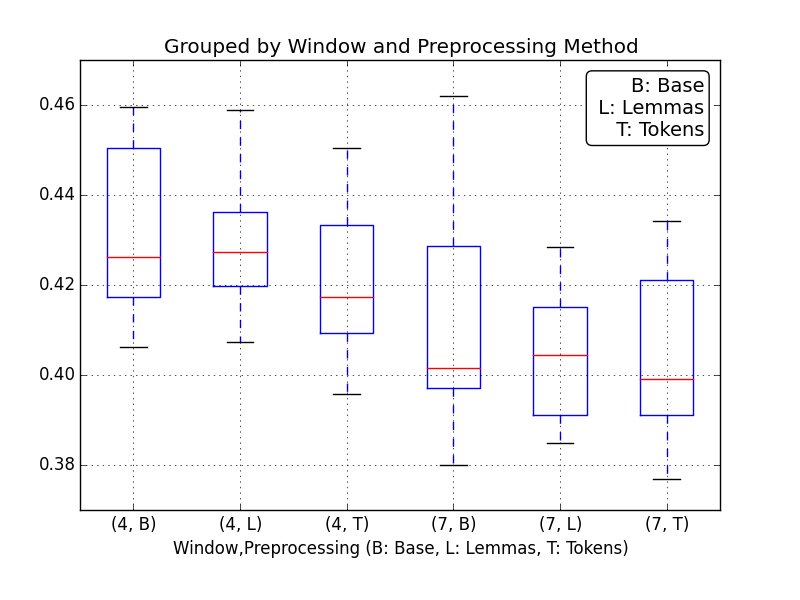
\includegraphics[width=\linewidth]{results_spearman/ar_similiarity_task_results_spearplot.png}
%   \caption{Results on Our Whole Arabic Task}
%   \label{fig:spearplot1}
% \end{wrapfigure}

% \begin{wrapfigure}{l}{0.5\linewidth}
%   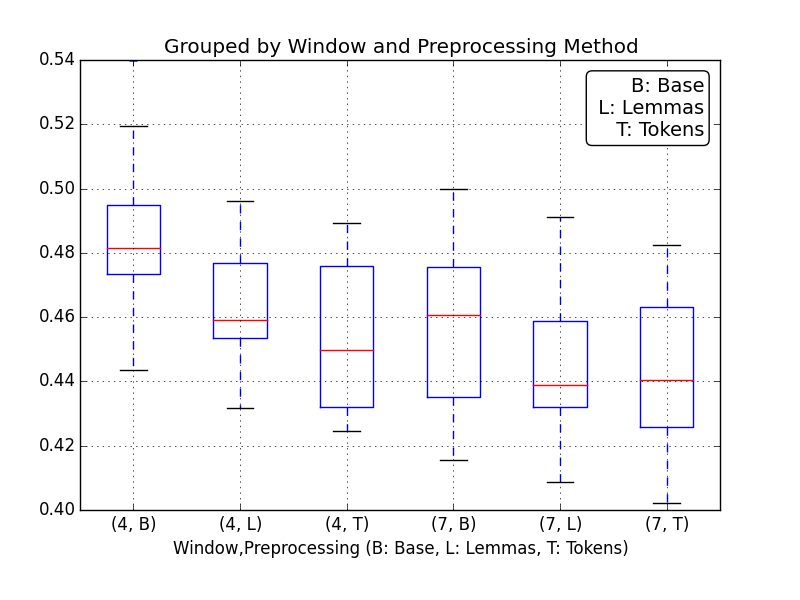
\includegraphics[width=\linewidth]{results_spearman/ar_similiarity_task_multi_results_spearplot.png}
%   \caption{Results on Our Arabic Task - 2+ Votes}
%   \label{fig:spearplot2}
% \end{wrapfigure}




\subsection{Analogy Task}

The English baseline results for the analogy task are $0.04522$ using 5 million training word Wikipedia subset and $0.73587$ using the 100 billion word Google News model. These results demonstrate the extreme difference in quality between vectors trained on 5 million words and 100 billion words. The lower accuracy of the 5 million word model at $0.04522$, or 4.522 percent correct of the $19544$ analogies, will be used as a comparitive baseline for this task. While this seems like a small percentage to attempt to improve, improving on this smaller scale is significant for a number of reasons. First, word embeddings have been shown to directly improve with data, so obtaining improvements without more data demonstrates an improvement in methodology, provided the improvements are not random luck \cite{mikolovdist:2013}. Secondly, improvements on the analogy task are nearly impossible to obtain through chance. To correctly solve just one of the hundreds of analogies, the embeddings must exactly guess the fourth word given the other three. This means the model must choose one word correctly from its entire Arabic vocabulary. Finally, as the results show, we examine a number of similar models and find results to be fairly consistent across a single parameter. While a larger set of training data would surely increase our percentages, we are confident that improvements on the smaller models will scale to larger training data. For these reasons, we leave training on a larger model as future work and continue our discussion of Arabic word embeddings in general terms.

\begin{wrapfigure}{l}{0.5\linewidth}
  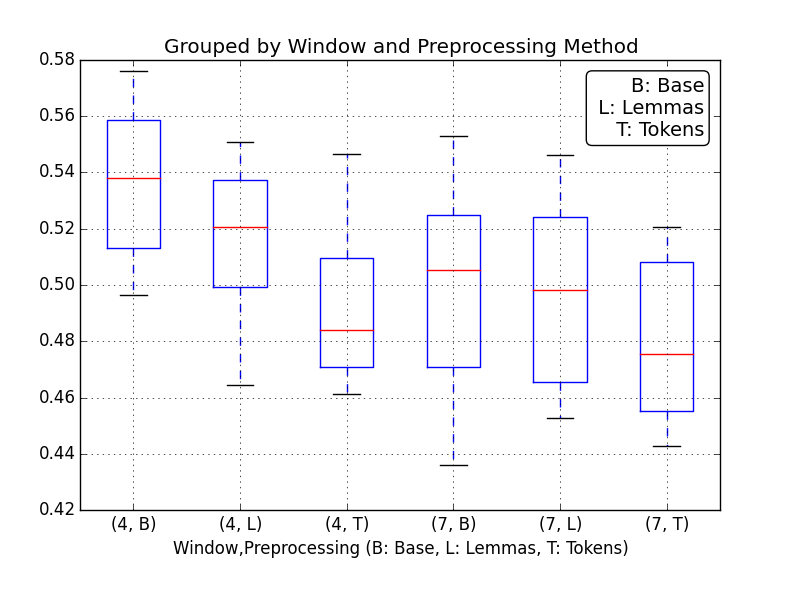
\includegraphics[width=\linewidth]{results_spearman/ar_similiarity_task_4_votes_results_spearplot.png}
  \caption{Results on Our Arabic Task - 4 Votes}
  \label{fig:spearplot4}
\end{wrapfigure}

Figure \ref{fig:aranalogy} shows the analogy task results from the Arabic models. Here it seems models preprocessed to lemmas and trained to 200 dimensions seem to dominate. This figure illustrates the dramatic improvements that are obtained with proper preprocessing and parameterization for the task. The lemmatized 200 dimensional models consistently outperformed all other models, including the baseline English model. In the best case, one ideally parameterized model is nearly 50\% better than the English baseline. Of lesser note, the tokenization method also delivers significantly higher accuracies than the models that received no preprocessing on the Arabic. These results demonstrate that preprocessing and training decisions can greatly improve the performance of Arabic word embeddings on analogy solving tasks, improving scores from as low as half of the English baseline to as high as 150\% of the baseline.

\begin{wrapfigure}{l}{0.5\linewidth}
  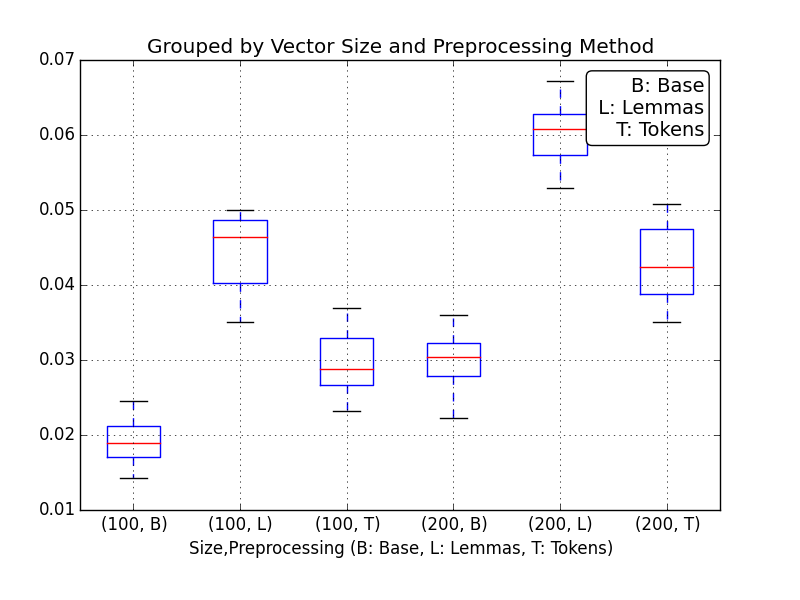
\includegraphics[width=\linewidth]{results_analogy/ar_analogy_results_fixed_plot.png}
  \caption{Arabic Analogy Task Results}
  \label{fig:aranalogy}
\end{wrapfigure}

% NEW EXPERIMENT HERE!


% \begin{wraptable}{l}{0.5\linewidth}
% \begin{center}
% \begin{tabular}{l|l}
% \bfseries Model & \bfseries Accuracy
% \csvreader[head to column names]{results_analogy/en_prepared.csv}{}
% {\\\hline\csvcoli&\csvcoliii}
% \end{tabular}
% \caption{English Analogy Results}
% \label{table:englishanalogy}
% \end{center}
% \end{wraptable}

% Embedding File,Hit_Percent,Scores,wind,size,mod,dig,tash,preprocessing
% 1               2           3      4   5      6 7    8   9


% \begin{wraptable}{l}{0.5\linewidth}
% \begin{center}
% \begin{tabular}{l|l|l|l|l}
% \bfseries Rank & \bfseries Preprocessing & \bfseries Window & \bfseries Size & \bfseries Accuracy
% \csvreader[head to column names]{results_analogy/ar_analogy_results_fixed_prepared.csv}{}
% {\\\hline\rank&\csvcolix&\csvcoliv&\csvcolv&\csvcoliii}
% \end{tabular}
% \caption{Top Results on Arabic Analogy Task}
% \label{table:aranalogy}
% \end{center}
% \end{wraptable}
















